\documentclass[a4paper,11pt,fleqn]{article}%fleqn pour aligner les equations à gauche
\usepackage{/home/rweye/Nextcloud/Documents/Overleaf/Styles/cours}

\newcommand{\chnum}{Chapitre 8}
\newcommand{\chtitle}{Synthèse d'un savon}
\newcommand{\dtype}{TP}
  


\begin{document}
	\maketitle
	
	
	\section{Fabrication à l'ancienne d'un savon}
Le savon est une substance liquide ou solide dont on retrouve les premières utilisations 3000 ans avant J.-C. Sa fabrication et son implication dans l'hygiène corporelle ne s'est développée en Europe pendant l'Antiquité. La fabrication du savon utilise alors des graisses animales ainsi que ses substances alcalines (cendres, herbes ...).\\
La méthode la plus courante pour leur fabrication utilise de l'hydroxyde de sodium (ou soude). La réaction chimique mise en jeu est appelée \emph{saponification} et peut s'écrire de la manière suivante :
$$\mathbf{\text{{huile d'olive}} + \text{soude} \rightarrow \text{savon} + \text{glycérol}}$$

La technique dure plus d'une semaine et comprend les quatre phases suivantes :
\begin{enumerate}
	\item \textbf{L'empâtage :} consistant à mettre en présence l'huile et la soude et à les mélanger en les faisant bouillir en présence d'eau dans une cuve pour qu'elles réagissent ensemble
	\item \textbf{Le relargage :} les deux produits formés sont séparés lors de l'opération dite de relargage en ajoutant de l'eau salée. L'ensemble se divise en deux couches. La partie inférieure, mélangée avec de l'eau, est retirée par le fond du chaudron à travers une tubulure
	\item \textbf{La cuisson :} la pâte de savon restant dans le chaudron est chauffée à ébullition pendant de nombreuses heures avec un excès de soude pour compléter la transformation
	\item \textbf{Les lavages :} éliminent l'excès de soude restant dans le savon ainsi que le glycérol et les impuretés.
\end{enumerate}
\noindent \begin{minipage}[t]{.5\linewidth}

	Enfin, la pâte chaude de savon est sortie de la cuve pour être étendue sur une feuille de papier, afin qu'elle refroidisse et perde une partie de son eau.\\
	En chimie, chaque synthèse comporte toujours quatre grandes étapes : 
	\begin{itemize}
		\item La \textbf{transformation chimique} proprement dite des réactifs en produits
		\item L'\textbf{isolement} du produit souhaité du mélange final dans lequel il se trouve
		\item La \textbf{purification} du produit obtenu
		\item L'\textbf{analyse} de la qualité du produit
	\end{itemize}	
\end{minipage}
\fbox{\begin{minipage}[t]{.5\linewidth}
	\begin{center}
		\textbf{Bilan de la réaction de saponification}\\ \vspace{2em}
		\begin{tabular}{cc>{\centering\arraybackslash}m{4cm}}
			\schemestart
			\chemfig[atom sep=2em]{CH_2(-[6]CH(-[6]CH_2 -O-CO-C_{17}H_{33})-O-CO-C_{17}H_{33})-O-CO-C_{17}H_{33}}
			\schemestop & + & \ce{3(Na+ + HO^-)}\\
			
			\textbf{Huile d'olve (Oléine)} & $\downarrow$ & \textbf{Hydroxyde de sodium (soude)}\\
			\schemestart
			\chemfig[atom sep=2em]{CH_2(-[6]CH(-[6]CH_2-OH)-OH)-OH}
			\schemestop 
			& + & \ce{3(Na+ + ^-O-CO-C17H33)} \\
			\textbf{Glycérol} & &\textbf{Savon}\\
		\end{tabular}
	\end{center}
\end{minipage}}


\begin{enumerate}
	\item Donner le nom et les formules brutes des réactifs et produits mis en jeu dans cette réaction.
	\item L'équation de la réaction est elle équilibrée ?
\end{enumerate}

\newpage
\section{Synthèse actuelle d'un savon}
La coude, ou hydroxyde de sodium, est un produit très corrosif et peut présenter un réel danger. Il est donc indispensable de manipuler avec la blouse fermée, les lunette de sécurité et les cheveux attachés.

\noindent\begin{minipage}{.5\linewidth}
Voici un protocole plus actuel permettant la synthèse d'un savon en laboratoire :
\begin{itemize}
	\item Retirer le ballon à fond rond du montage et le poser sur le valet sur la paillasse.
	\item Introduire dans le ballon le mélange réactionnel qui se compose de :
	\begin{itemize}
		\item \SI{8}{mL} d'huile alimentaire
		\item \SI{10}{mL} de solution de soude 
		\item \SI{10}{mL} d'éthanol
		\item 4 grains de pierre ponce (elle sert à réguler l'ébullition en formant des bulles de gaz plus petites)
	\end{itemize}
	\item Placer le ballon dans le chauffe-ballon, lui-même placé sur un support élévateur.
	\item Replacer le ballon sur le montage avec le réfrigérant à boules.
	\item Mettre en route la circulation d'eau dans le réfrigérant à boules.
	\item Régler le chauffe-ballon au 2/3 du chauffage maximal.
	\item Laisser la réaction se dérouler pendant au moins 20 minutes. Pendant ce temps, répondre aux questions.
\end{itemize}
\end{minipage}
\begin{minipage}{.5\linewidth}
	\begin{center}
		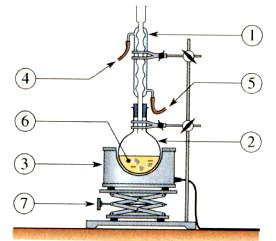
\includegraphics[width=\linewidth]{Ressources/2GT_C11_TP_Fig2.png}
	\end{center}
\end{minipage}

\begin{enumerate}[resume]
	\item Recopier les numéros du schéma précédent et y adjoindre l'annotation correspondante.
	\item A quoi sert la pierre ponce ?
	\item A quoi sert le réfrigérant à boules ?
	\item Quel est l'intérêt du montage à reflux ?
\end{enumerate}
\newpage
\section{Extraction du savon}
	\subsection{Étape de relargage}
	\begin{itemize}
		\item Au bout des 20 minutes, arrêter le chauffage et descendre le support élévateur. Laisser refroidir le ballon quelques minutes à l'air libre.\\
		\emph{Arrêter la circulation d'eau froide dans le réfrigérant}
		\item Pendant que le ballon refroidit, préparer \SI{60}{mL} d'eau très salée prélevés à l'éprouvette graduée et les verser dans le bécher.
		\item En vous aidant d'un chiffon, enlever le ballon et verser son contenu dans l'eau très salée du bécher.
		\item Ajouter environ \SI{20}{mL} d'eau froide du robinet.\\
		\emph{Le savon est soluble dans l'eau et très eu soluble dans l'eau salée}.
	\end{itemize}
	\subsection{Étape de filtration sous vide}
	\noindent \begin{minipage}{.5\linewidth}
		\begin{itemize}
			\item Placer un papier filtre rond dans l'entonnoir Büchner.
			\item verser un peu d'eau distillée sur le papier filtre rond pour l'humidifier de manière \textbf{homogène}. Il va ainsi "coller" à l'entonnoir.
			\item Ouvrir le robinet d'eau.\\
			\emph{La trompe à eau, par son appel d'air, crée une dépression dans l'erlenmeyer. Le mélange à filtrer est alors aspiré au travers du papier filtre.}
			\item Verser en plusieurs fois le contenu du bécher dans l'entonnoir Büchner.
		\end{itemize}
	\emph{Pendant la filtration, appuyer sur l'entonnoir avec la paume de la main, de façon à bine plaquer l'entonnoir et le joint contre l'erlenmeyer, pour assurer une bonne étanchéité.}
	\end{minipage}
	\begin{minipage}{.5\linewidth}
		\begin{center}
			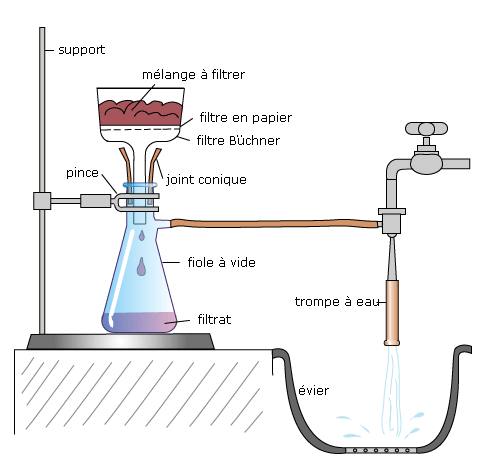
\includegraphics[width=\linewidth]{Ressources/2GT_C11_TP_Fig3.png}
		\end{center}
	\end{minipage}
	
\section{Questions :}
\begin{enumerate}[resume]
	\item Noter la masse de savon obtenue expérimentalement, $m_{exp}$.
	\item Calculer la quantité de matière obtenue expérimentalement, notée $n_{exp}$, sachant qu'une mole de savon a une masse de \SI{304,0}{g}.
	\item Calculer la masse d'oléine utilisée pour la réaction, sachant que la masse volumique de l'huile vaut $\rho_{huile}$ = \SI{0,92}{\gram\per\milli\liter}
	\item Sachant que la concentration de la solution d'hydroxyde de sodium introduite dans le mélange est de \SI{300}{\gram\per\liter}, déterminer le réactif limitant.
	\item À partir des données expérimentales, tenter de d'exprimer un rendement de la réaction.
\end{enumerate}
\textbf{Données :}
\begin{itemize}
	\item \textbf{Masse des atomes :} $m(O)$ = \SI{2,82E-23}{g}, $m(C)$ = \SI{2,11E-23}{g}, $m(H)$ = \SI{1,67E-24}{g}, $m(Na)$ = \SI{3,87E-23}{g}
	\item \textbf{Nombre d'Avogadro :} $N_A$ = \SI{6,02E-23}{\per\mole}
\end{itemize}
\end{document}

